\documentclass[11pt]{article}

\usepackage[margin=1in]{geometry}
\usepackage{graphicx}
\graphicspath{{figures/}}
\usepackage{booktabs}
\usepackage{amsmath,amssymb}
\usepackage{siunitx}
\usepackage{hyperref}
\usepackage{caption}
\usepackage{float}
\usepackage[numbers,sort&compress]{natbib}

\title{\textbf{Coherence, Topology, and Memory in DOFT Oscillator Networks: Scaling Laws and Testable Links to Vortex Matter in Type-II Superconductors}}
\author{C. Agostino\\\small Independent Researcher, Buenos Aires, Argentina}
\date{\today}

\begin{document}
\maketitle

\begin{abstract}
Delayed-Oscillator Field Theory (DOFT) models stable structure emerging from networks of coupled oscillators with finite delay and internal memory. We treat DOFT as a speculative but testable constraint-based program. Prior DOFT work reported discrete ``prime-space fingerprints'' and integer-participation structure extracted from superconducting materials datasets; here we shift to a DOFT-only simulation program to test whether comparable organization emerges intrinsically from DOFT dynamics.

We introduce a sequential multistage pipeline (Ola1--Ola4) that separates candidate search from dynamical measurement: a fast \emph{Explorer} proposes and filters candidate network instances, while a multicore \emph{Sweep} integrates the governing delayed dynamics and computes late-time observables. Across network sizes $N=2$--$12$ and several template families (rings, ladders, bipartites, complete graphs), three findings organize the results: (i) mean global coherence decreases monotonically with $N$, consistent in this range with a geometric decay $R\propto N^{-b}$ with $b\approx 0.32\pm 0.03$ (also compatible with relaxation toward a finite floor); (ii) at larger $N$, surviving outcomes exhibit elevated participation of a distinct memory layer ($S2$), suggesting memory acts as a stabilization overhead under geometric stress; (iii) topology becomes increasingly selective with $N$, with a transition region around $N\approx 6$--$9$ culminating in an apparent ceiling near $N\approx 8$--$9$ for monolithic templates where survival rates collapse.

We propose a falsifiable bridge to vortex matter in type-II superconductors: if DOFT coherence behaves like an order/correlation proxy and network size maps monotonically to vortex density, then the observed exponent and regime changes can be compared quantitatively to field-dependent ordering lengths in collective pinning and vortex melting phenomenology \citep{Abrikosov1957,LarkinOvchinnikov1979,Blatter1994}. This correspondence is framed as a testable hypothesis, not an identification.
\end{abstract}

\textbf{Keywords:} delayed oscillators; coherence scaling; topology selection; memory layer; structural ceiling; vortex lattice; collective pinning; Abrikosov lattice; order--disorder transition.

\section{Introduction}

\subsection{Constraints before Hamiltonians}
Delayed-Oscillator Field Theory (DOFT) takes a constraint-first starting point: instead of deriving structure from a microscopic Hamiltonian, it asks what stable patterns are permitted by delayed coupling, finite internal memory, and the requirement that oscillators can form stable locks. This ``allowed vs.\ probable'' view produces falsifiable predictions (scaling laws, selection rules, phase boundaries) without requiring a full microscopic mapping.

\subsection{From phenomenological signatures to intrinsic dynamics}
Earlier DOFT work reported discrete signatures (prime-indexed organizational patterns and integer-dominated participation) extracted from superconducting materials datasets. A key open question is whether such structure is intrinsic to DOFT dynamics or an artifact of mapping DOFT observables onto external data. This paper isolates the intrinsic mechanism by studying DOFT in a simulation-only setting.

\subsection{Why vortex matter is a concrete interface}
Type-II superconductors under field provide a well-characterized testbed where increasing vortex density drives transitions from ordered Abrikosov lattices to disordered phases. These transitions are probed via SANS, $\mu$SR, real-space imaging, and transport anomalies. We use this as a quantitative interface: if an empirical mapping between DOFT complexity and vortex density holds, then DOFT scaling exponents and regime boundaries become directly testable.

\section{Computational Framework: the Ola Pipeline}

\subsection{Explorer vs.\ Sweep}
Scaling DOFT studies faces combinatorial growth in candidate networks. We separate (i) a fast Explorer that proposes candidates from topology templates and a growing library of promoted building blocks, from (ii) a slow Sweep that performs numerical integration and measures late-time observables. All quantitative results in this paper come from Sweep outputs.

\subsection{Ola1--Ola4 stages and thresholds}
The pipeline proceeds through four stages (Ola1--Ola4), each expanding $N$ and tightening selection thresholds for computational tractability. Because thresholds vary by stage, raw promoted counts are not directly comparable across olas; we therefore emphasize within-template rates and common-threshold replots (Appendix \ref{app:common-threshold}).

\section{Definitions and Observables}

\subsection{Global coherence $R$}
We measure global coherence as a phase-order parameter in $[0,1]$ computed over the last window of each run:
\begin{equation}
R(t)=\left|\frac{1}{N}\sum_{j=1}^{N}e^{i\theta_j(t)}\right|,\qquad
\bar{R}=\langle R(t)\rangle_{\text{last window}}.
\end{equation}
Higher $R$ corresponds to stronger global synchronization.

\subsection{Memory participation $S2$}
We report memory participation as $S2$ share (a normalized fraction of late-time participation/energy associated with the memory layer). Operationally, this is computed from Sweep-logged layer contributions and averaged over the last window.

\subsection{Topology templates and outcome labels}
Candidates are generated from fixed template families (rings, ladders, bipartites, complete graphs). Runs are labeled as \emph{survivors} (promoted) or \emph{failures} (evaluated but not promoted), using stage-specific thresholds.

\section{Results}

\subsection{Coherence decays geometrically with network size}
Figure~\ref{fig:coherence-scaling} shows that mean coherence decreases monotonically with network size. Over $N=2$--$12$, a power law fit yields $R\propto N^{-b}$ with $b\approx 0.32$ (CI width $\sim 0.03$), consistent with an exponent near $1/3$.

\begin{figure}[H]
\centering
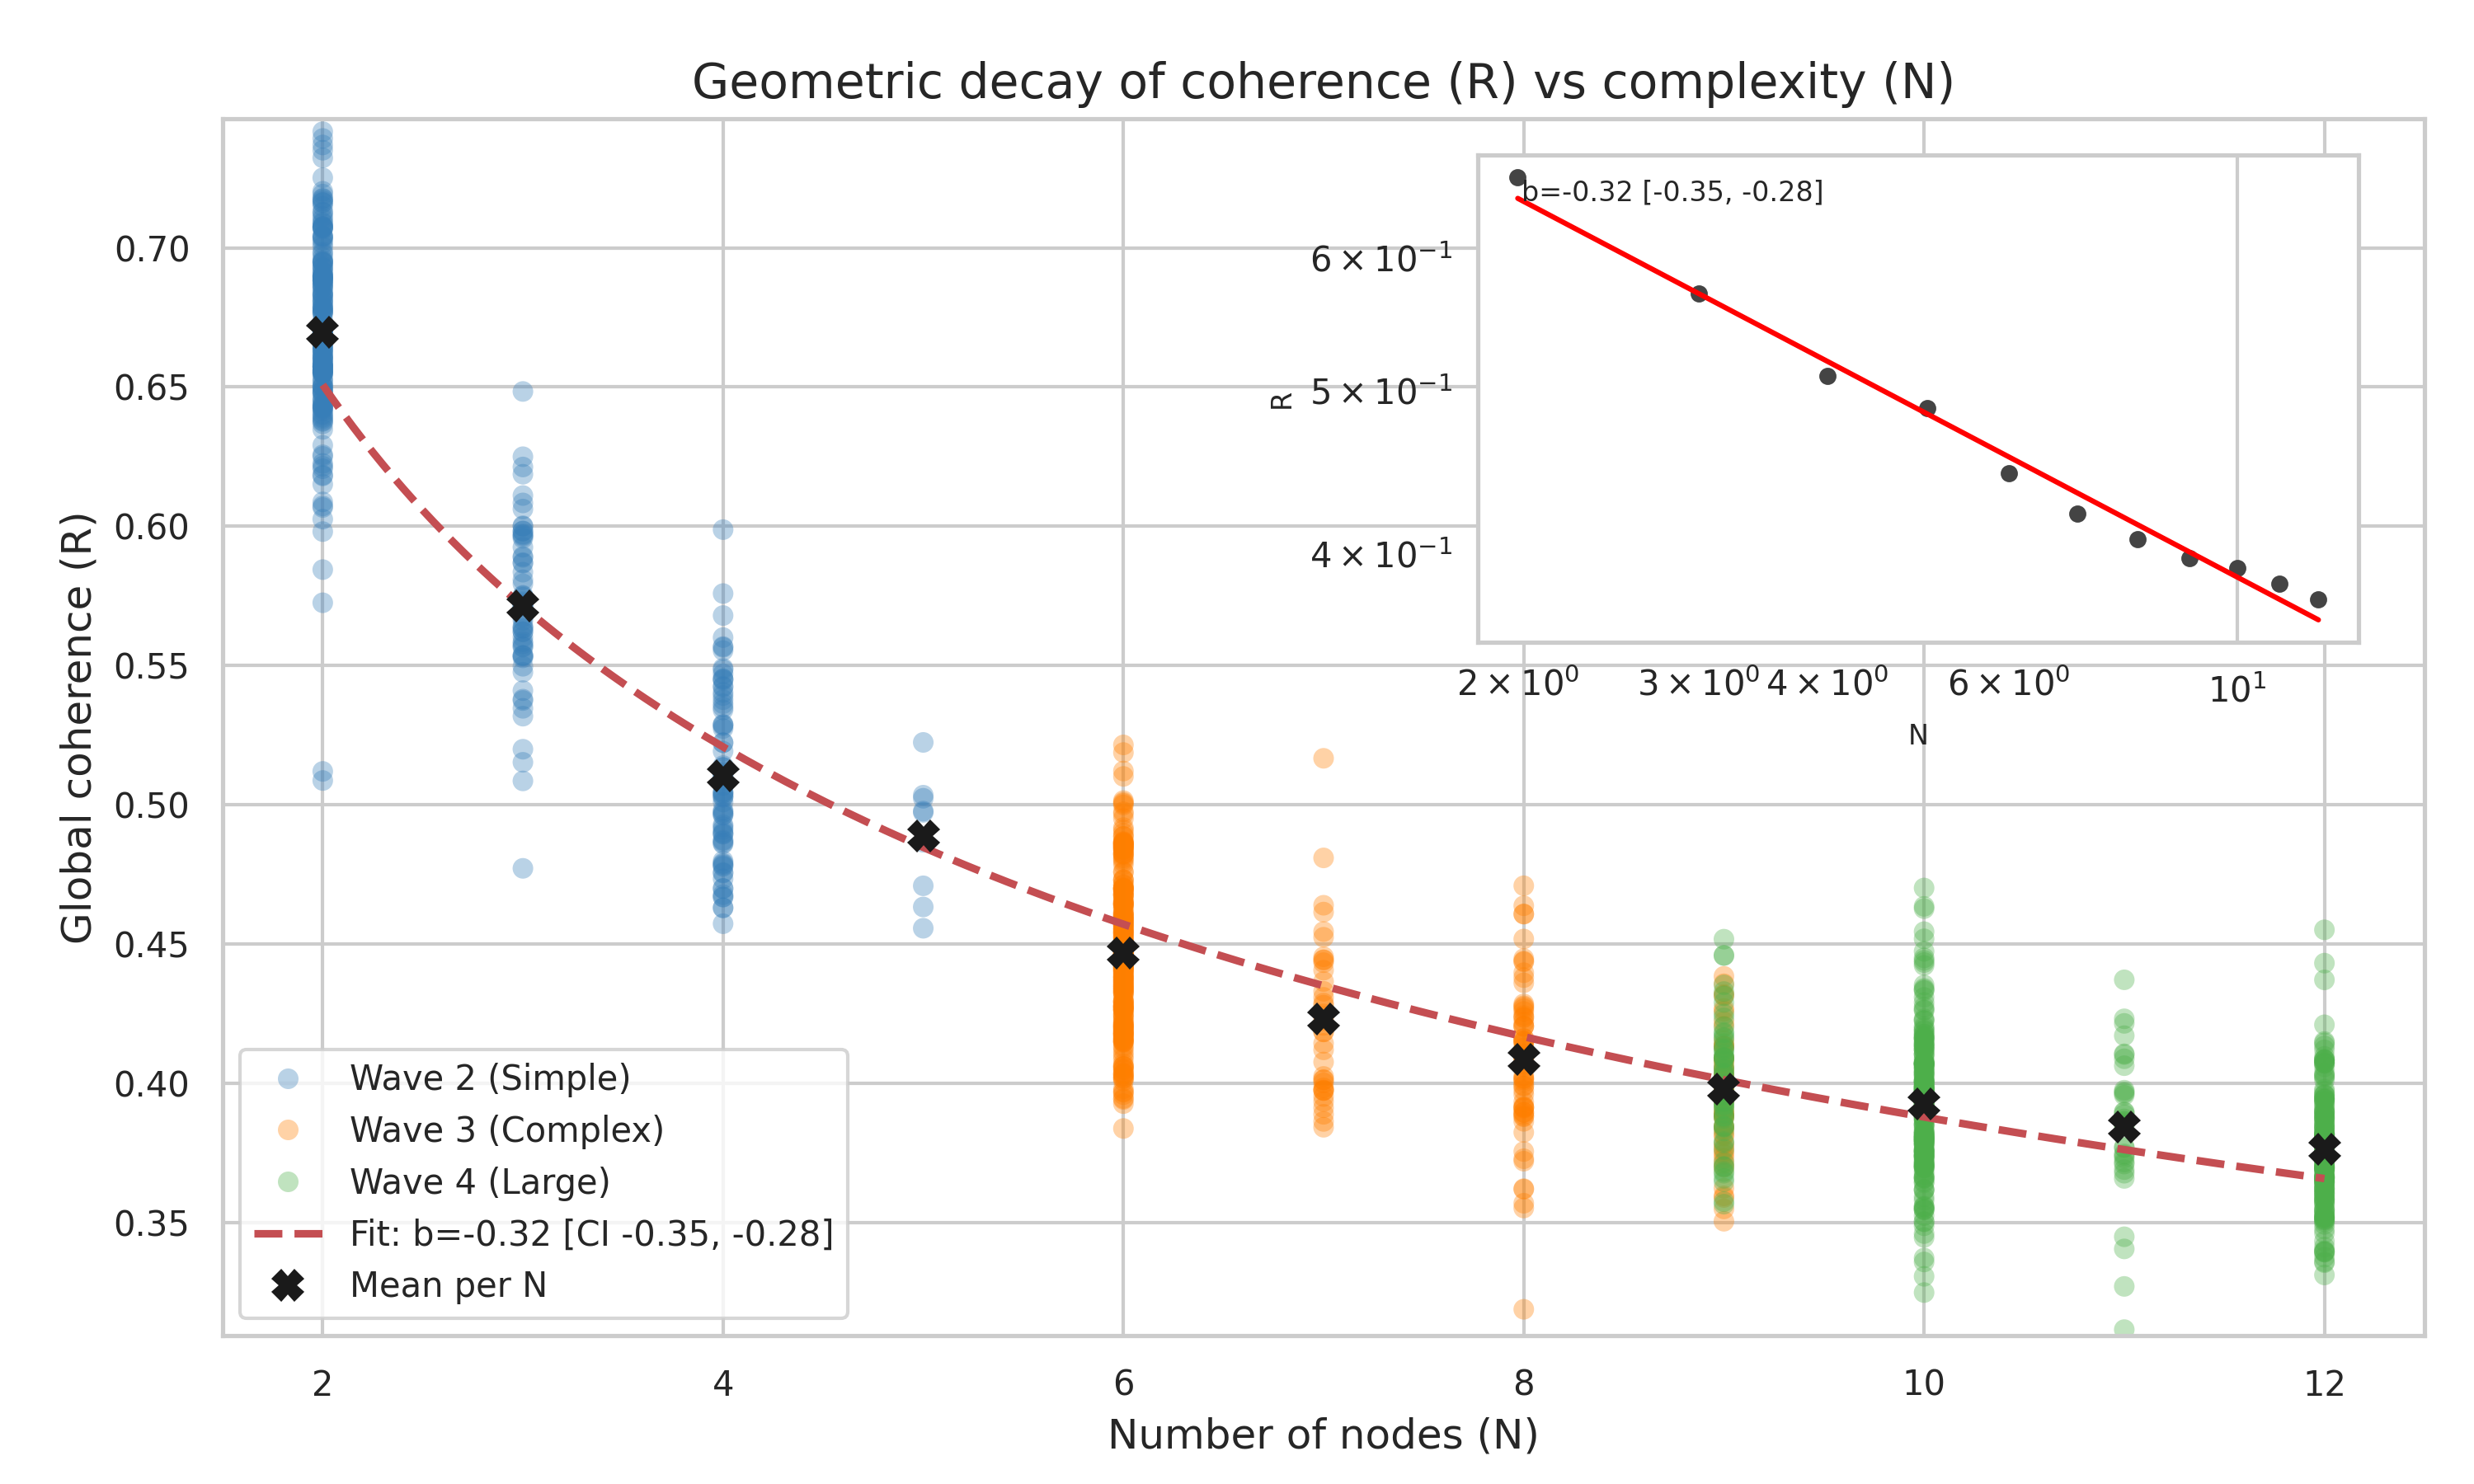
\includegraphics[width=\linewidth]{Figure_1_Coherence_Scaling.png}
\caption{Global coherence $R$ vs.\ network size $N$ across runs and stages. Dashed curve: power-law fit. Inset: log--log view.}
\label{fig:coherence-scaling}
\end{figure}

\subsection{Memory overhead emerges under geometric stress}
Figure~\ref{fig:memory-overhead} shows $S2$ participation vs.\ $N$ split by outcome. At small $N$ failures are rare and $S2$ is low; at larger $N$, survivors cluster at elevated $S2$ share, consistent with memory acting as stabilization overhead.

\begin{figure}[H]
\centering
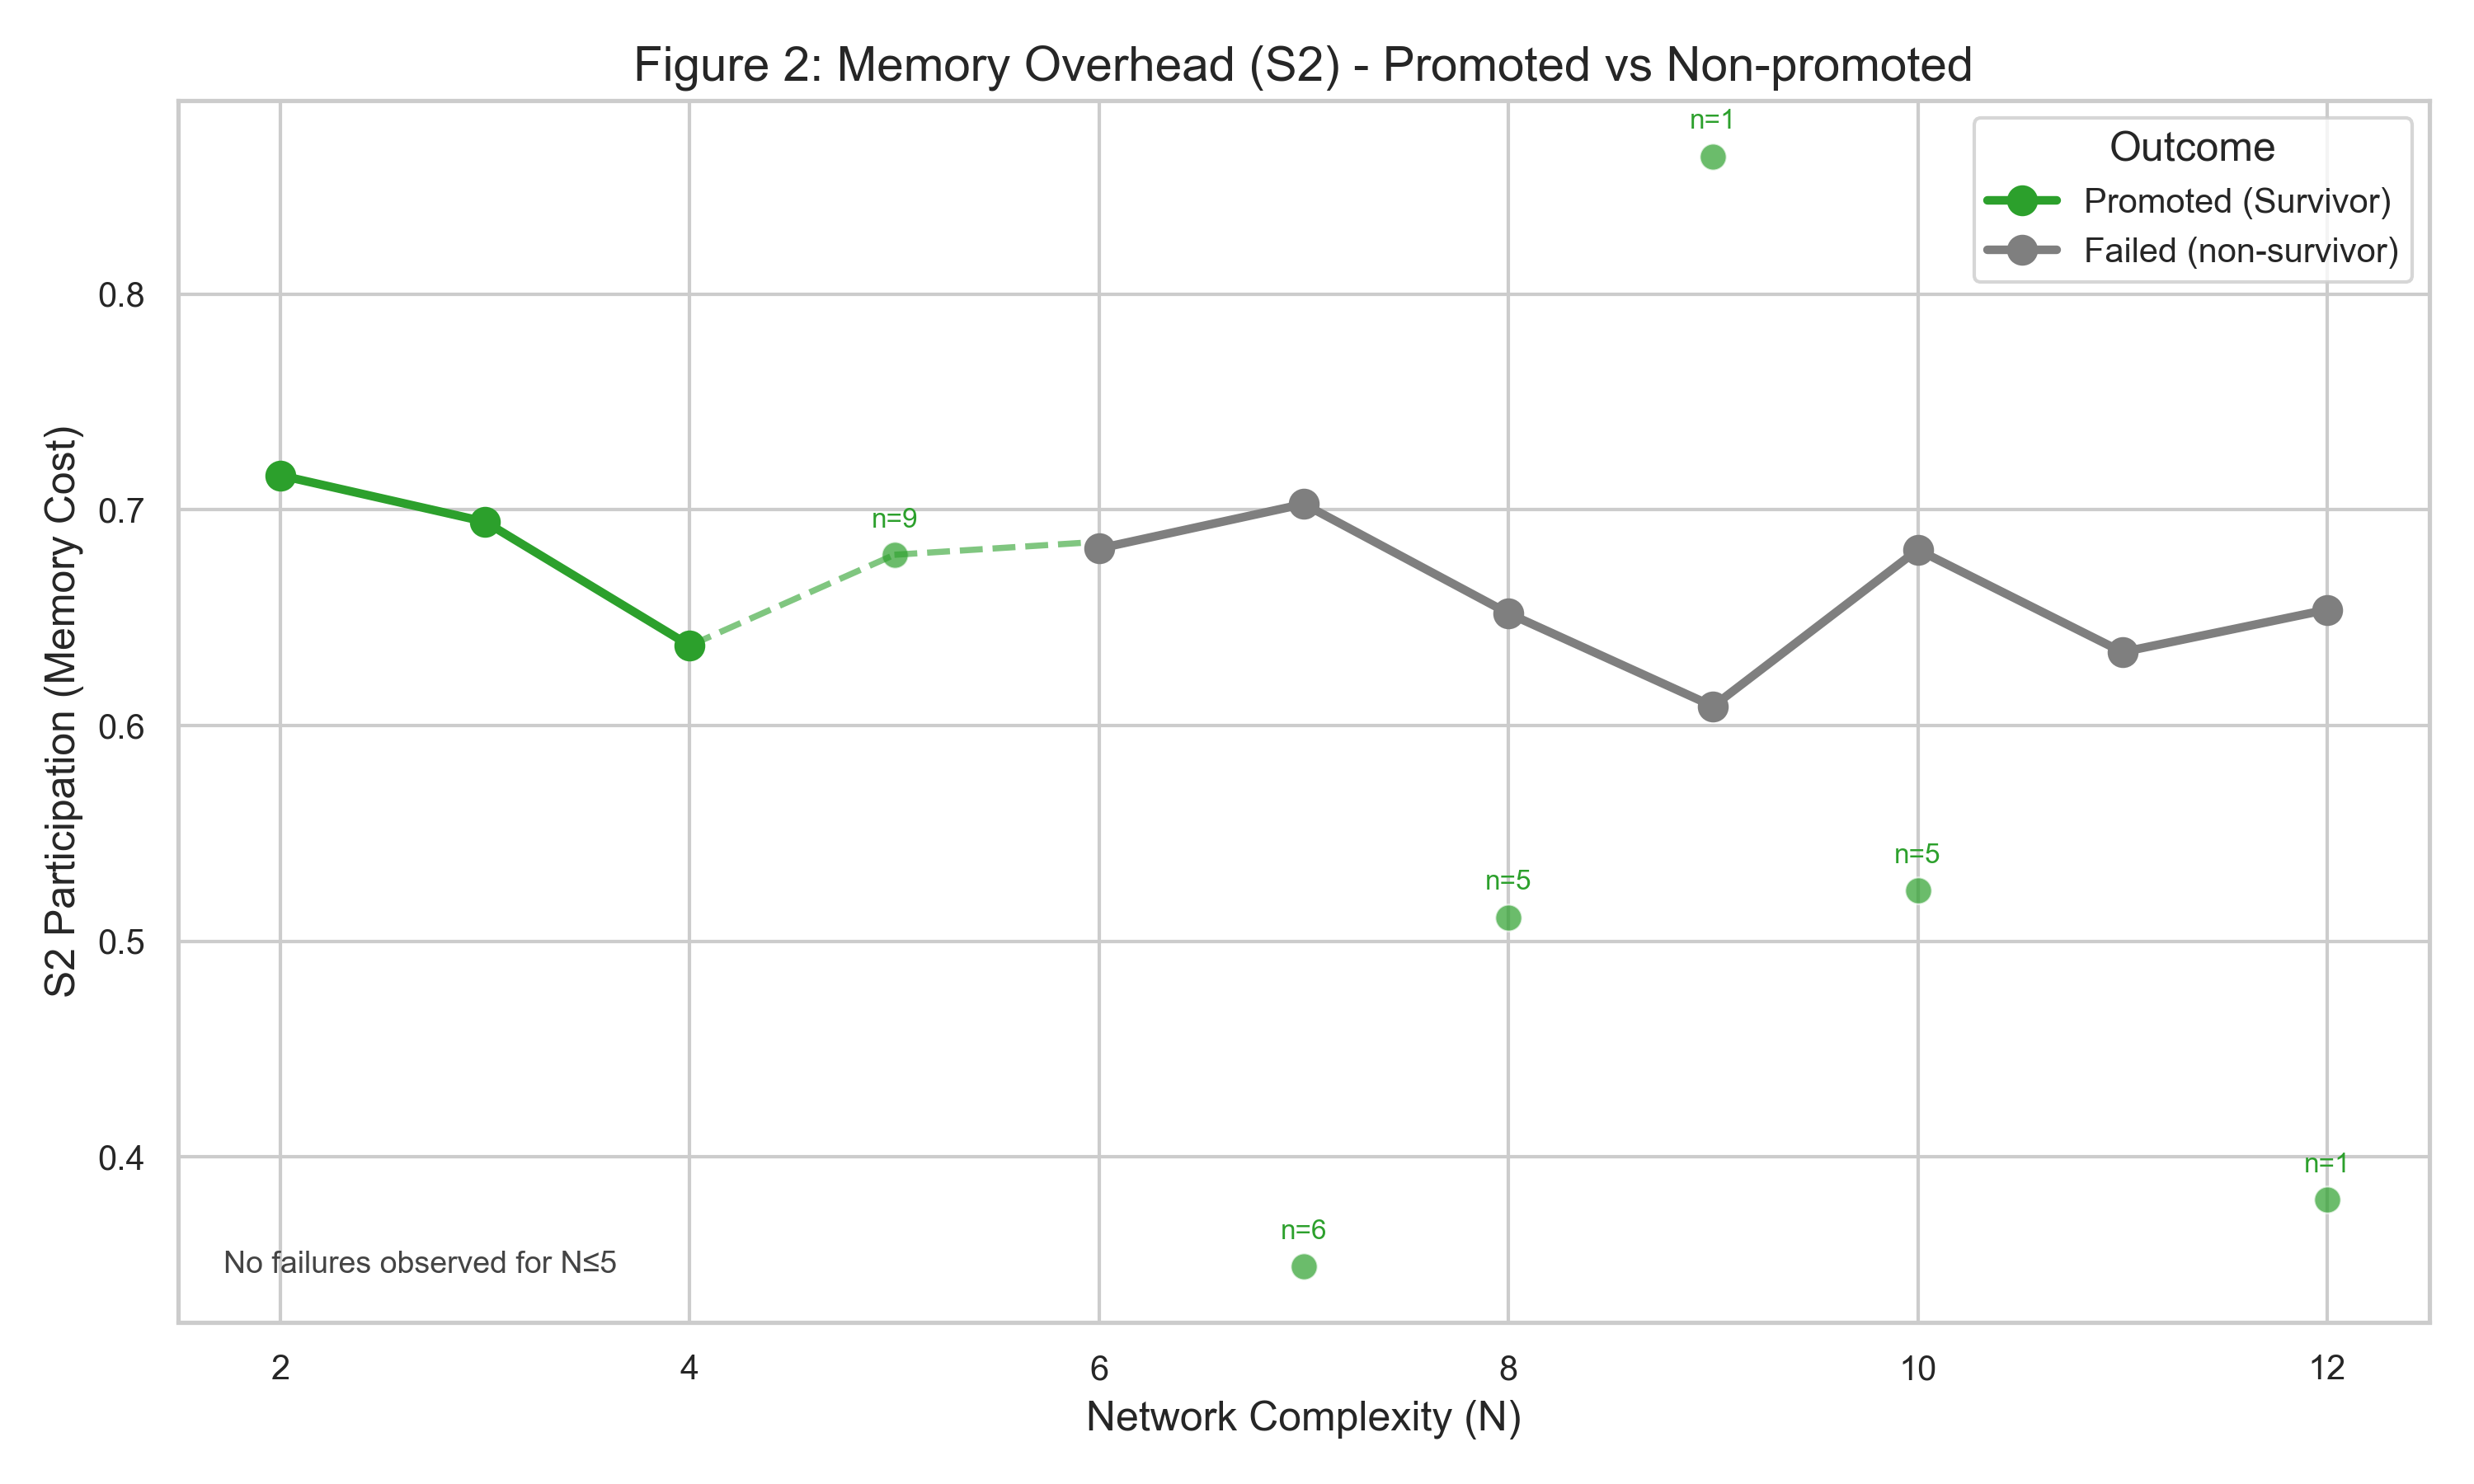
\includegraphics[width=\linewidth]{Figure_2_Memory_Overhead.png}
\caption{$S2$ participation (memory cost) vs.\ $N$, split by outcome (promoted vs.\ non-survivor).}
\label{fig:memory-overhead}
\end{figure}

\subsection{Topology becomes selective: monolithic templates hit a ceiling}
Figure~\ref{fig:topology-ceiling} summarizes success rates by template and $N$ under a fixed coherence threshold. Monolithic templates (rings/ladders) show a sharp collapse near $N\approx 8$--$9$, while modular templates (bipartites) retain viability at larger $N$.

\begin{figure}[H]
\centering
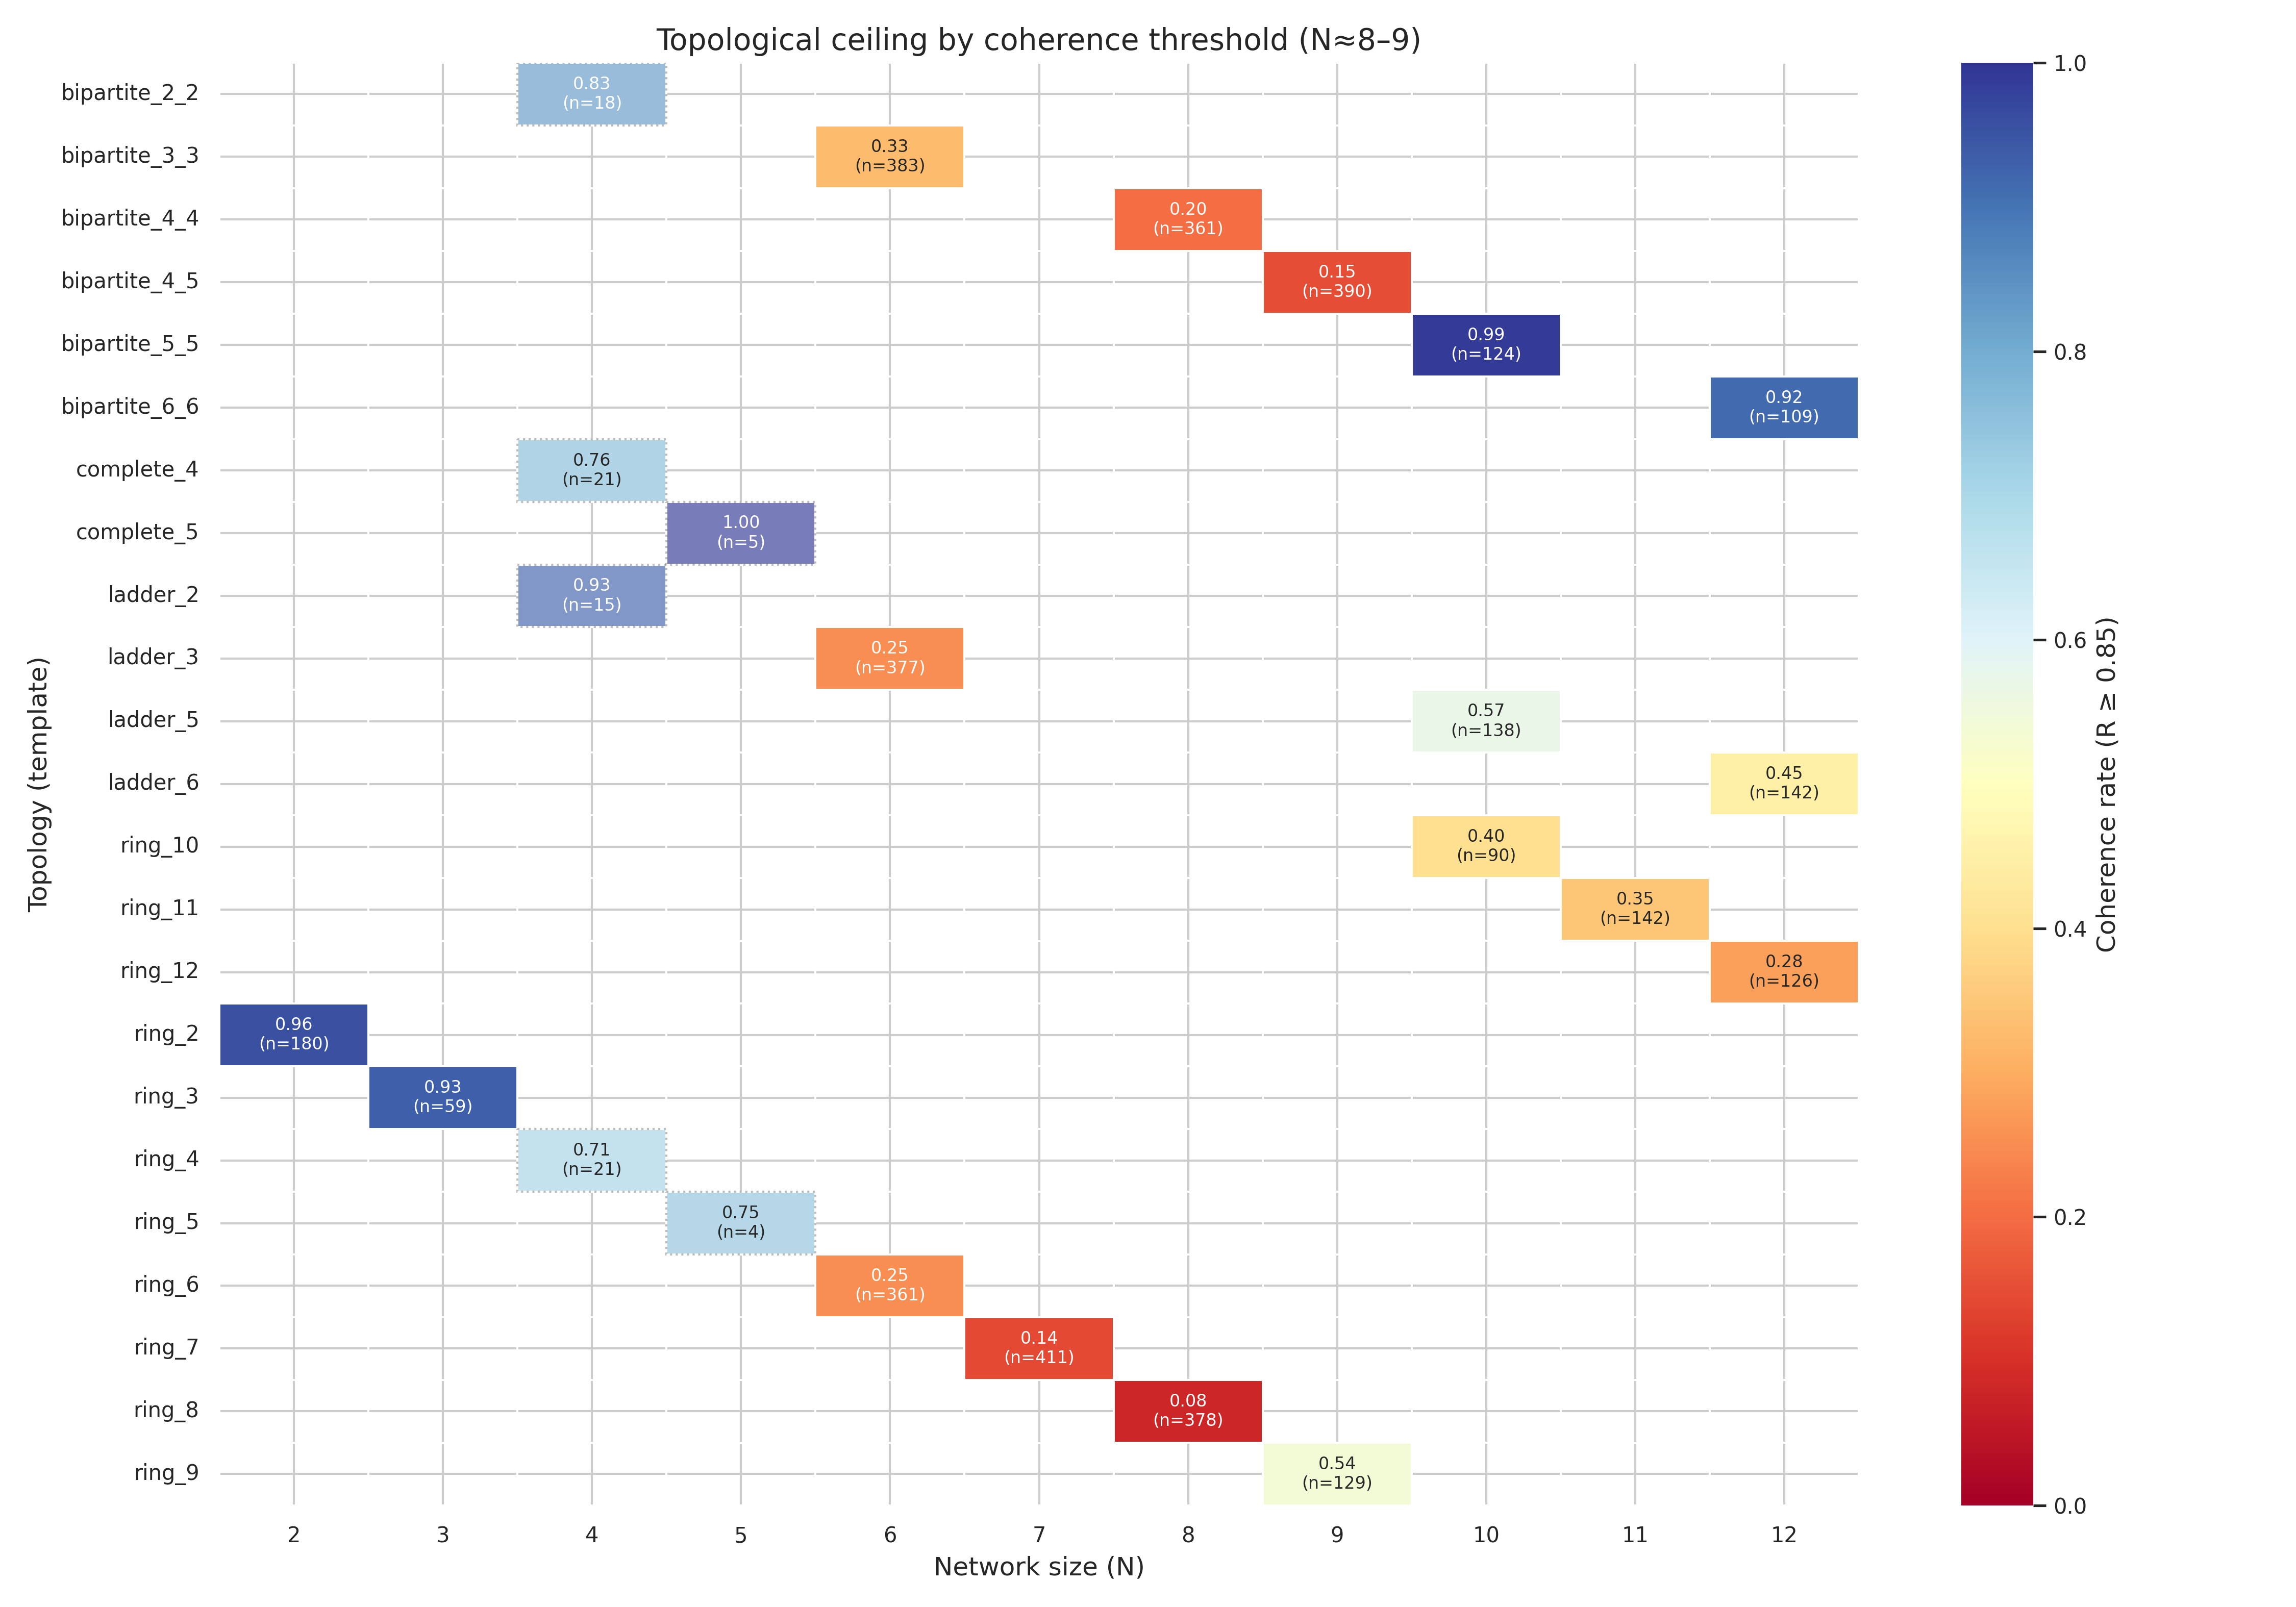
\includegraphics[width=\linewidth]{Figure_3_Topology_Ceiling.png}
\caption{Template-conditioned coherence ``ceiling'' under a common threshold (as annotated in the figure). Colors indicate coherence rate; each cell reports sample size $n$.}
\label{fig:topology-ceiling}
\end{figure}

\subsection{Mechanism check: memory does not linearly drive coherence}
To decouple size effects, we compute coherence residuals within-$N$ and regress them on $S2$. Figure~\ref{fig:mechanism-check} shows a near-zero slope (CI crosses zero), indicating $S2$ is better interpreted as a viability requirement at large $N$ rather than a direct linear driver of higher coherence.

\begin{figure}[H]
\centering
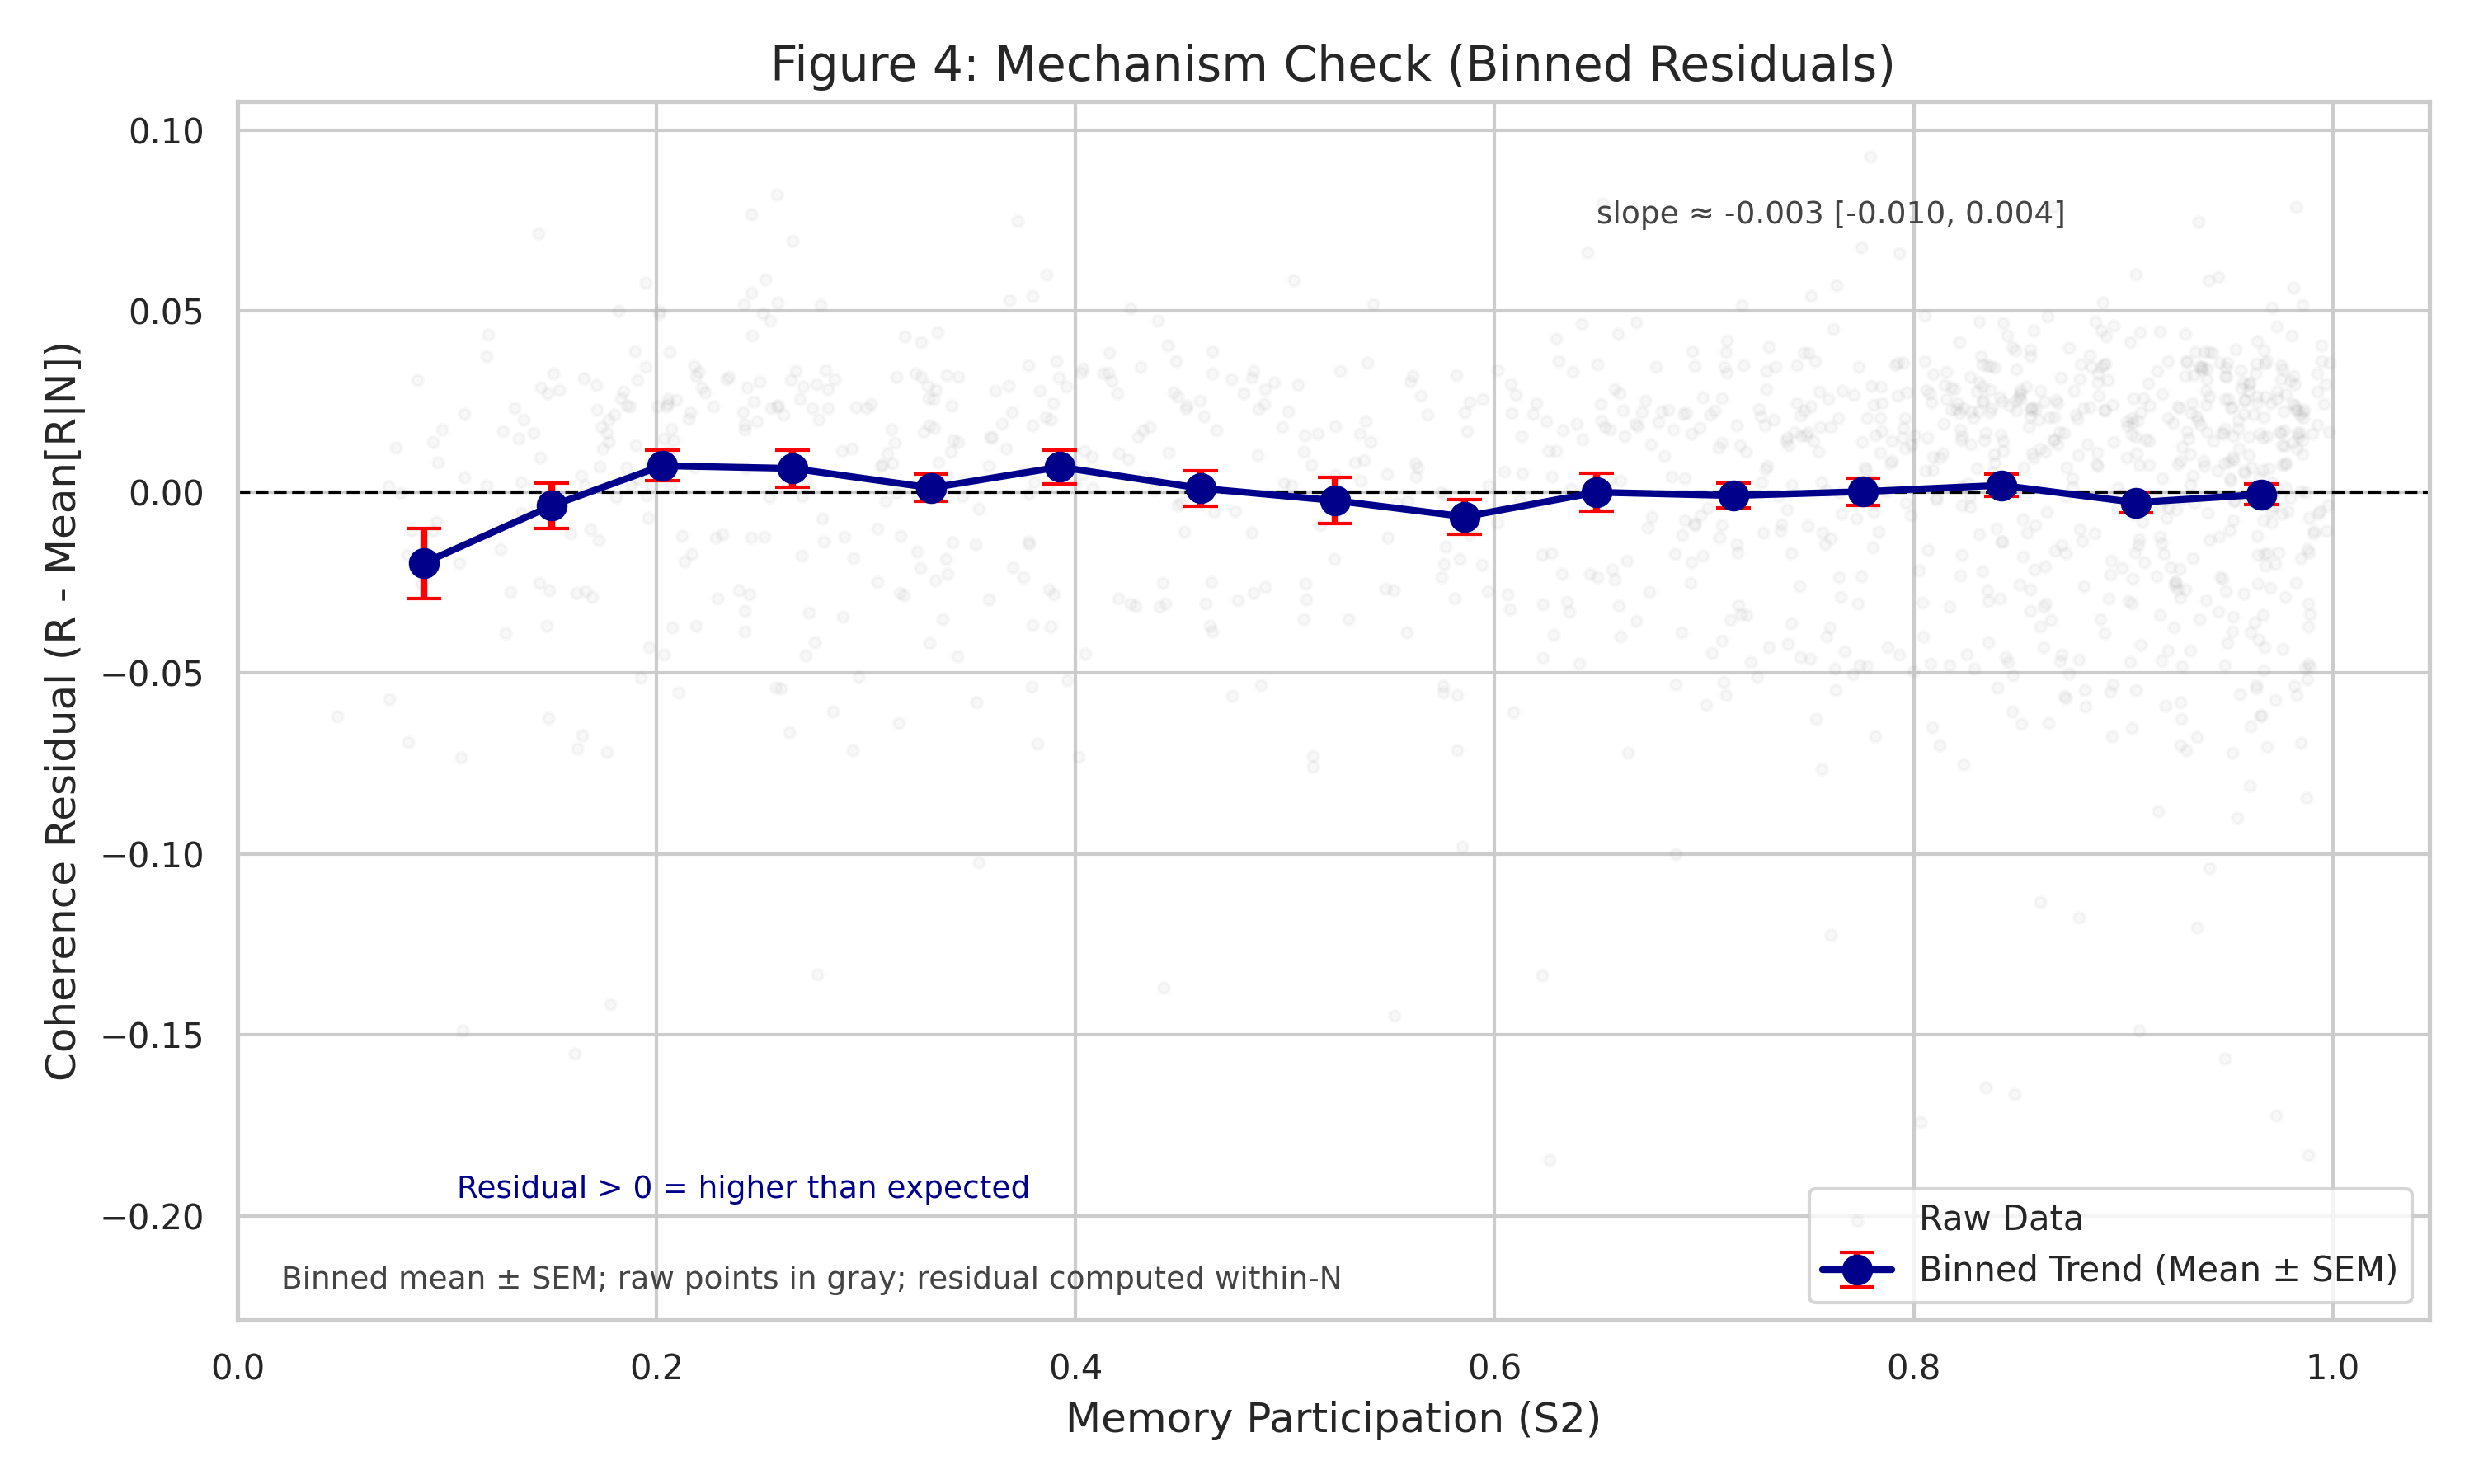
\includegraphics[width=\linewidth]{Figure_4_Mechanism_Binned.png}
\caption{Within-$N$ coherence residual vs.\ $S2$ participation (binned mean $\pm$ SEM with raw points).}
\label{fig:mechanism-check}
\end{figure}

\section{Discussion}

\subsection{What the scaling law does and does not claim}
The exponent $b\approx 0.32$ is an empirical regularity extracted from simulations; we do not derive it from DOFT axioms. Within the probed range it compresses the dominant trend: coherence degrades systematically as $N$ increases.

\subsection{Memory as compensation, not cognition}
$S2$ is a dynamical slow degree of freedom, not a learning or control algorithm. The observed regime dependence (overhead at low $N$, necessity at high $N$) suggests a compensation channel that becomes relevant when geometric coordination becomes fragile.

\subsection{A falsifiable bridge to vortex matter}
Vortex matter in type-II superconductors exhibits field-dependent ordering lengths and order--disorder transitions \citep{Abrikosov1957,Blatter1994}. Collective pinning approaches (e.g.\ Larkin--Ovchinnikov) provide regimes with distinct scaling behaviors \citep{LarkinOvchinnikov1979,GiamarchiLeDoussal1994}. We propose the bridge as a testable hypothesis: if a monotone mapping between DOFT complexity and vortex density is defensible for a chosen experimental regime, then (i) the exponent range and (ii) regime boundaries/role reversals can be compared to experimental correlation proxies. This bridge is falsified by persistent exponent mismatch or by absence of comparable regime changes in the targeted experimental window.

\section{Conclusion}
Using a DOFT-only simulation pipeline (Ola1--Ola4), we find (i) monotone coherence decay consistent in this range with $R\propto N^{-1/3}$, (ii) elevated memory participation among large-$N$ survivors consistent with stabilization overhead, and (iii) increasing topology selectivity culminating in a ceiling for monolithic templates near $N\approx 8$--$9$. We provide appendices with additional diagnostics and recommend targeted comparisons to vortex matter as falsifiable tests.

\section*{Data and Code Availability}
For Zenodo packaging: include the analysis notebooks used to generate each figure, per-stage CSV/JSON exports, and an exact code snapshot (commit hash) of the Explorer/Sweep engines. Provide a single \texttt{reproduce.sh} (or \texttt{make}) entry point that regenerates all figures from raw exports.

\bibliographystyle{unsrtnat}
\bibliography{references}

\appendix

\section{Common-threshold replots and selection confounds}
\label{app:common-threshold}
Stage-specific thresholds are used for tractability. To reduce confounds, we recommend reporting (i) within-template success rates at fixed $N$, and (ii) replots under a common coherence threshold wherever sample sizes permit.

\section{Within-$N$ Spearman correlation: $S2$ vs.\ coherence}
\label{app:spearman}
Figure~\ref{fig:spearman} shows the within-$N$ Spearman correlation between $S2$ participation and coherence. The sign change across $N$ supports a regime boundary interpretation.

\begin{figure}[H]
\centering
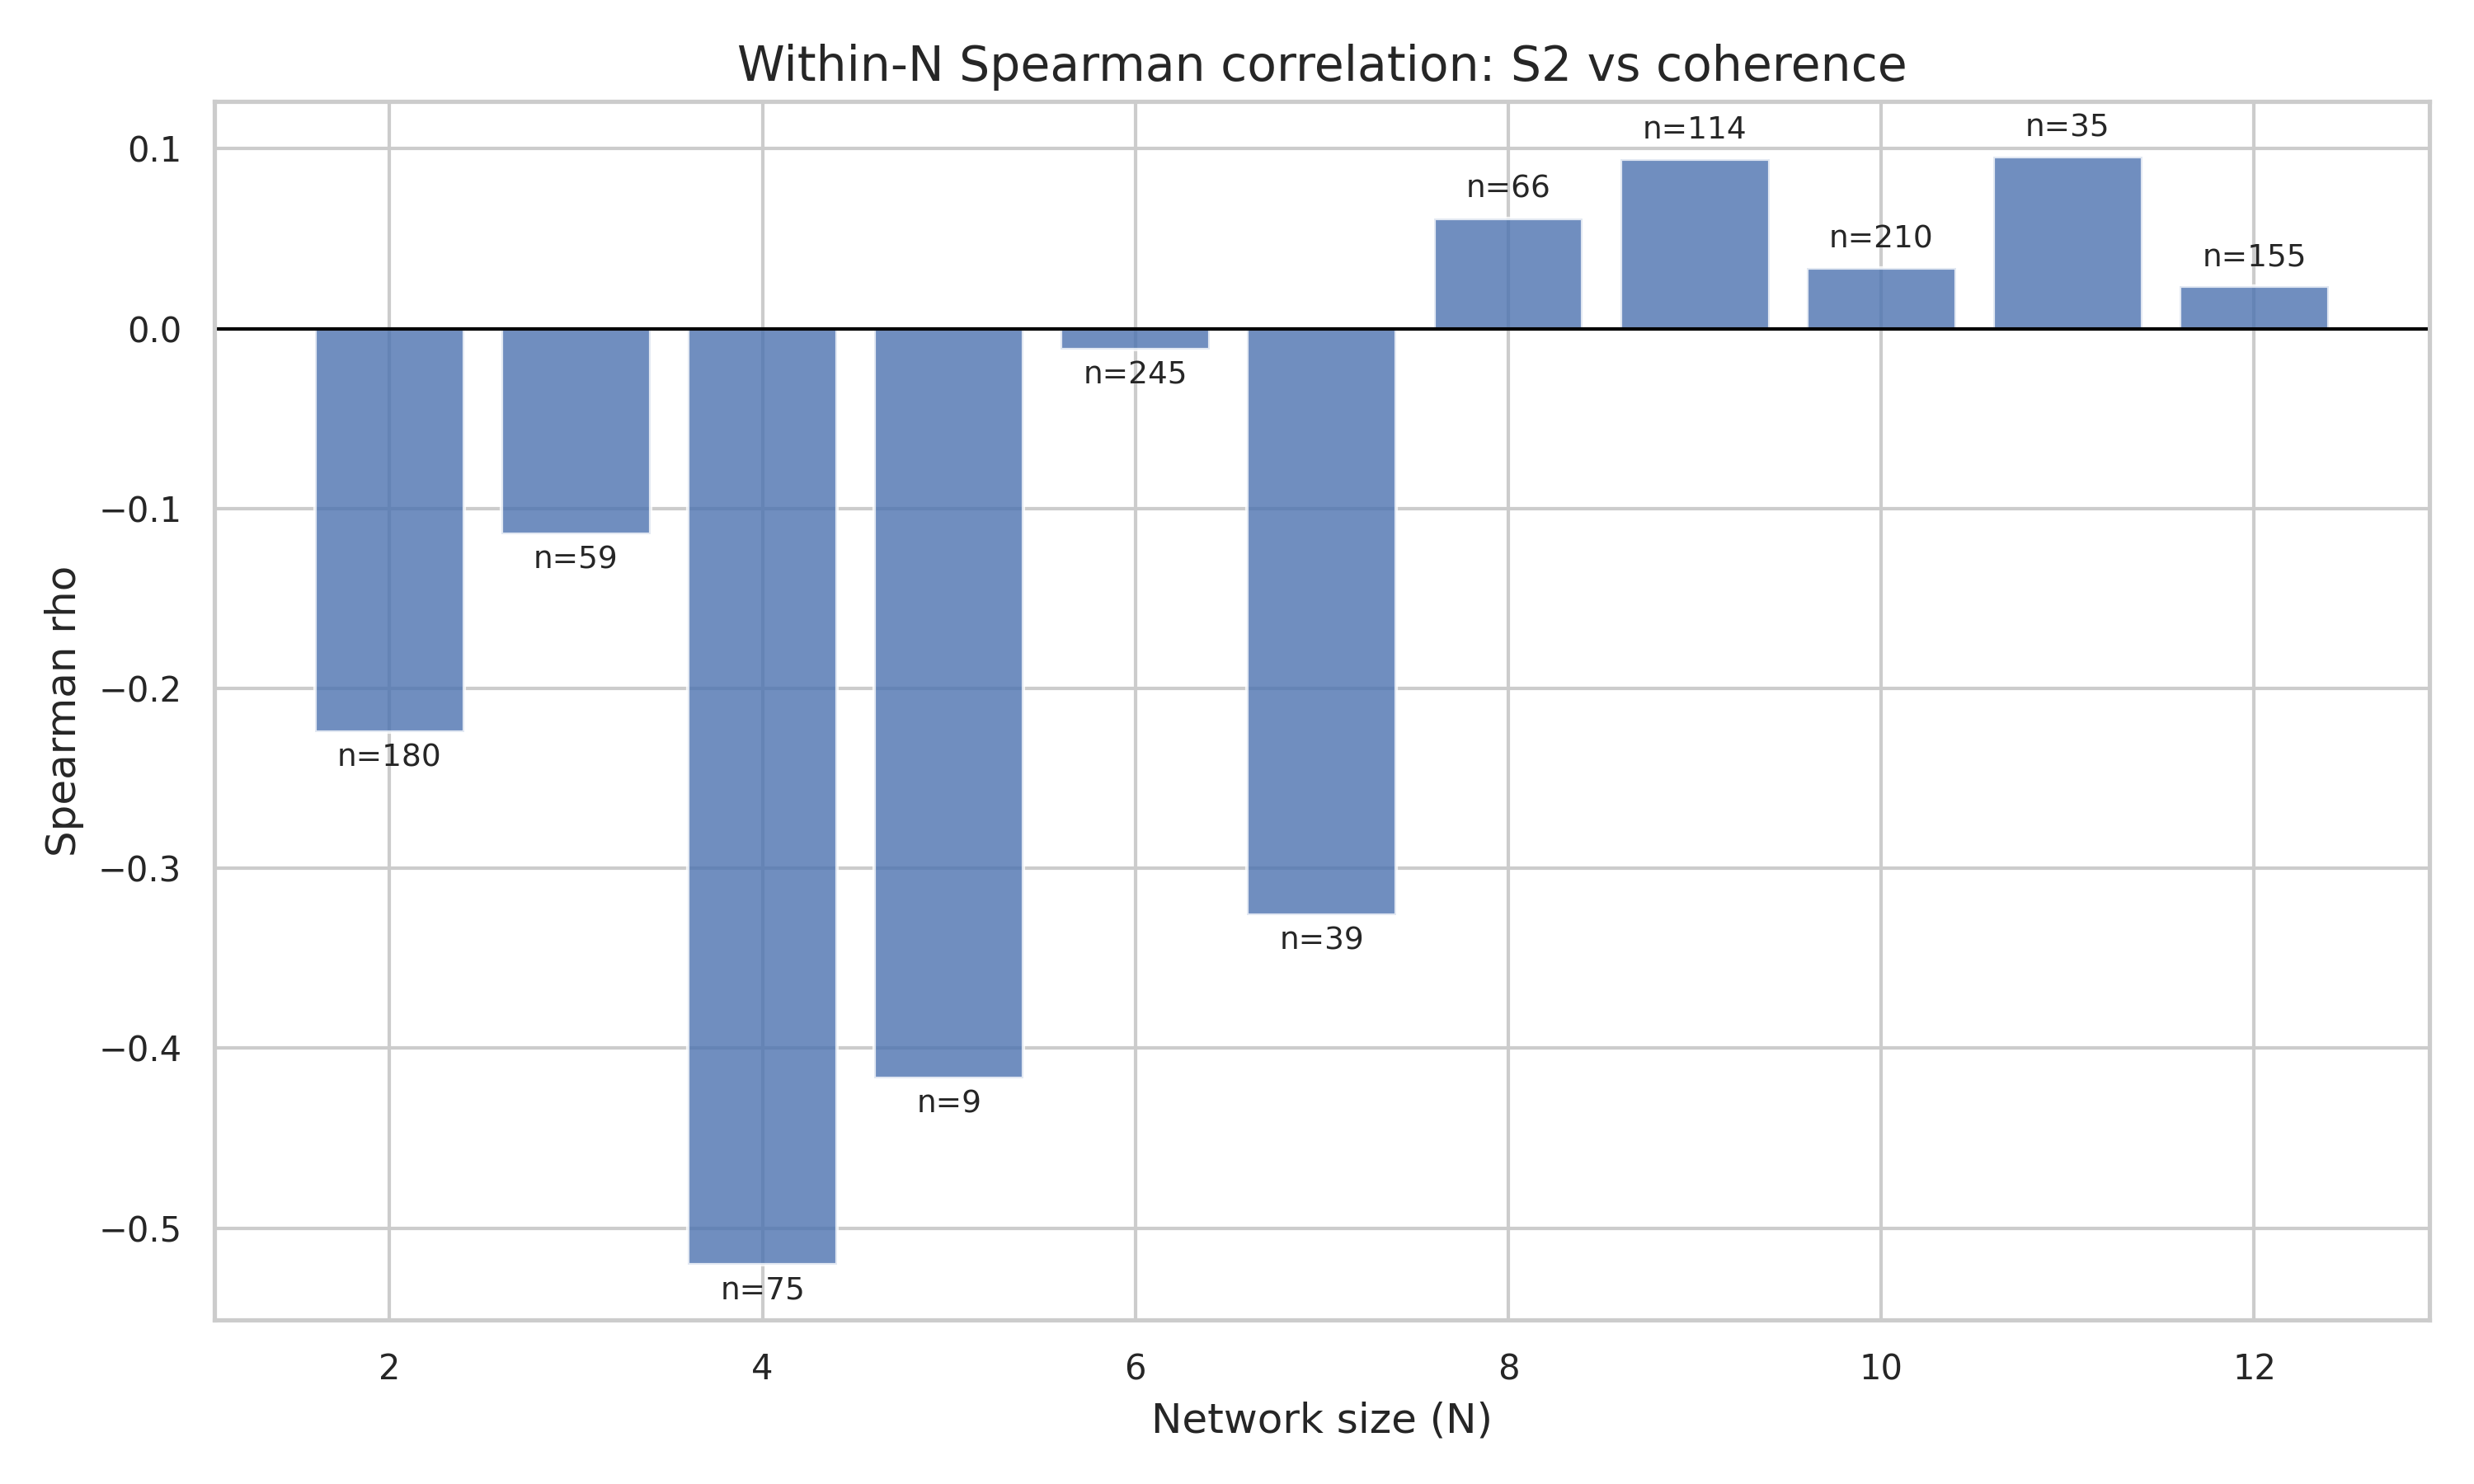
\includegraphics[width=\linewidth]{Appendix_C_spearman_rho_by_n.png}
\caption{Within-$N$ Spearman correlation between $S2$ and coherence (with sample sizes).}
\label{fig:spearman}
\end{figure}

\section{Fluctuation peak diagnostics}
\label{app:fluct}
Figure~\ref{fig:fluct} reports dispersion measures vs.\ $N$ (IQR-based diagnostics) used to identify a fluctuation peak regime.

\begin{figure}[H]
\centering
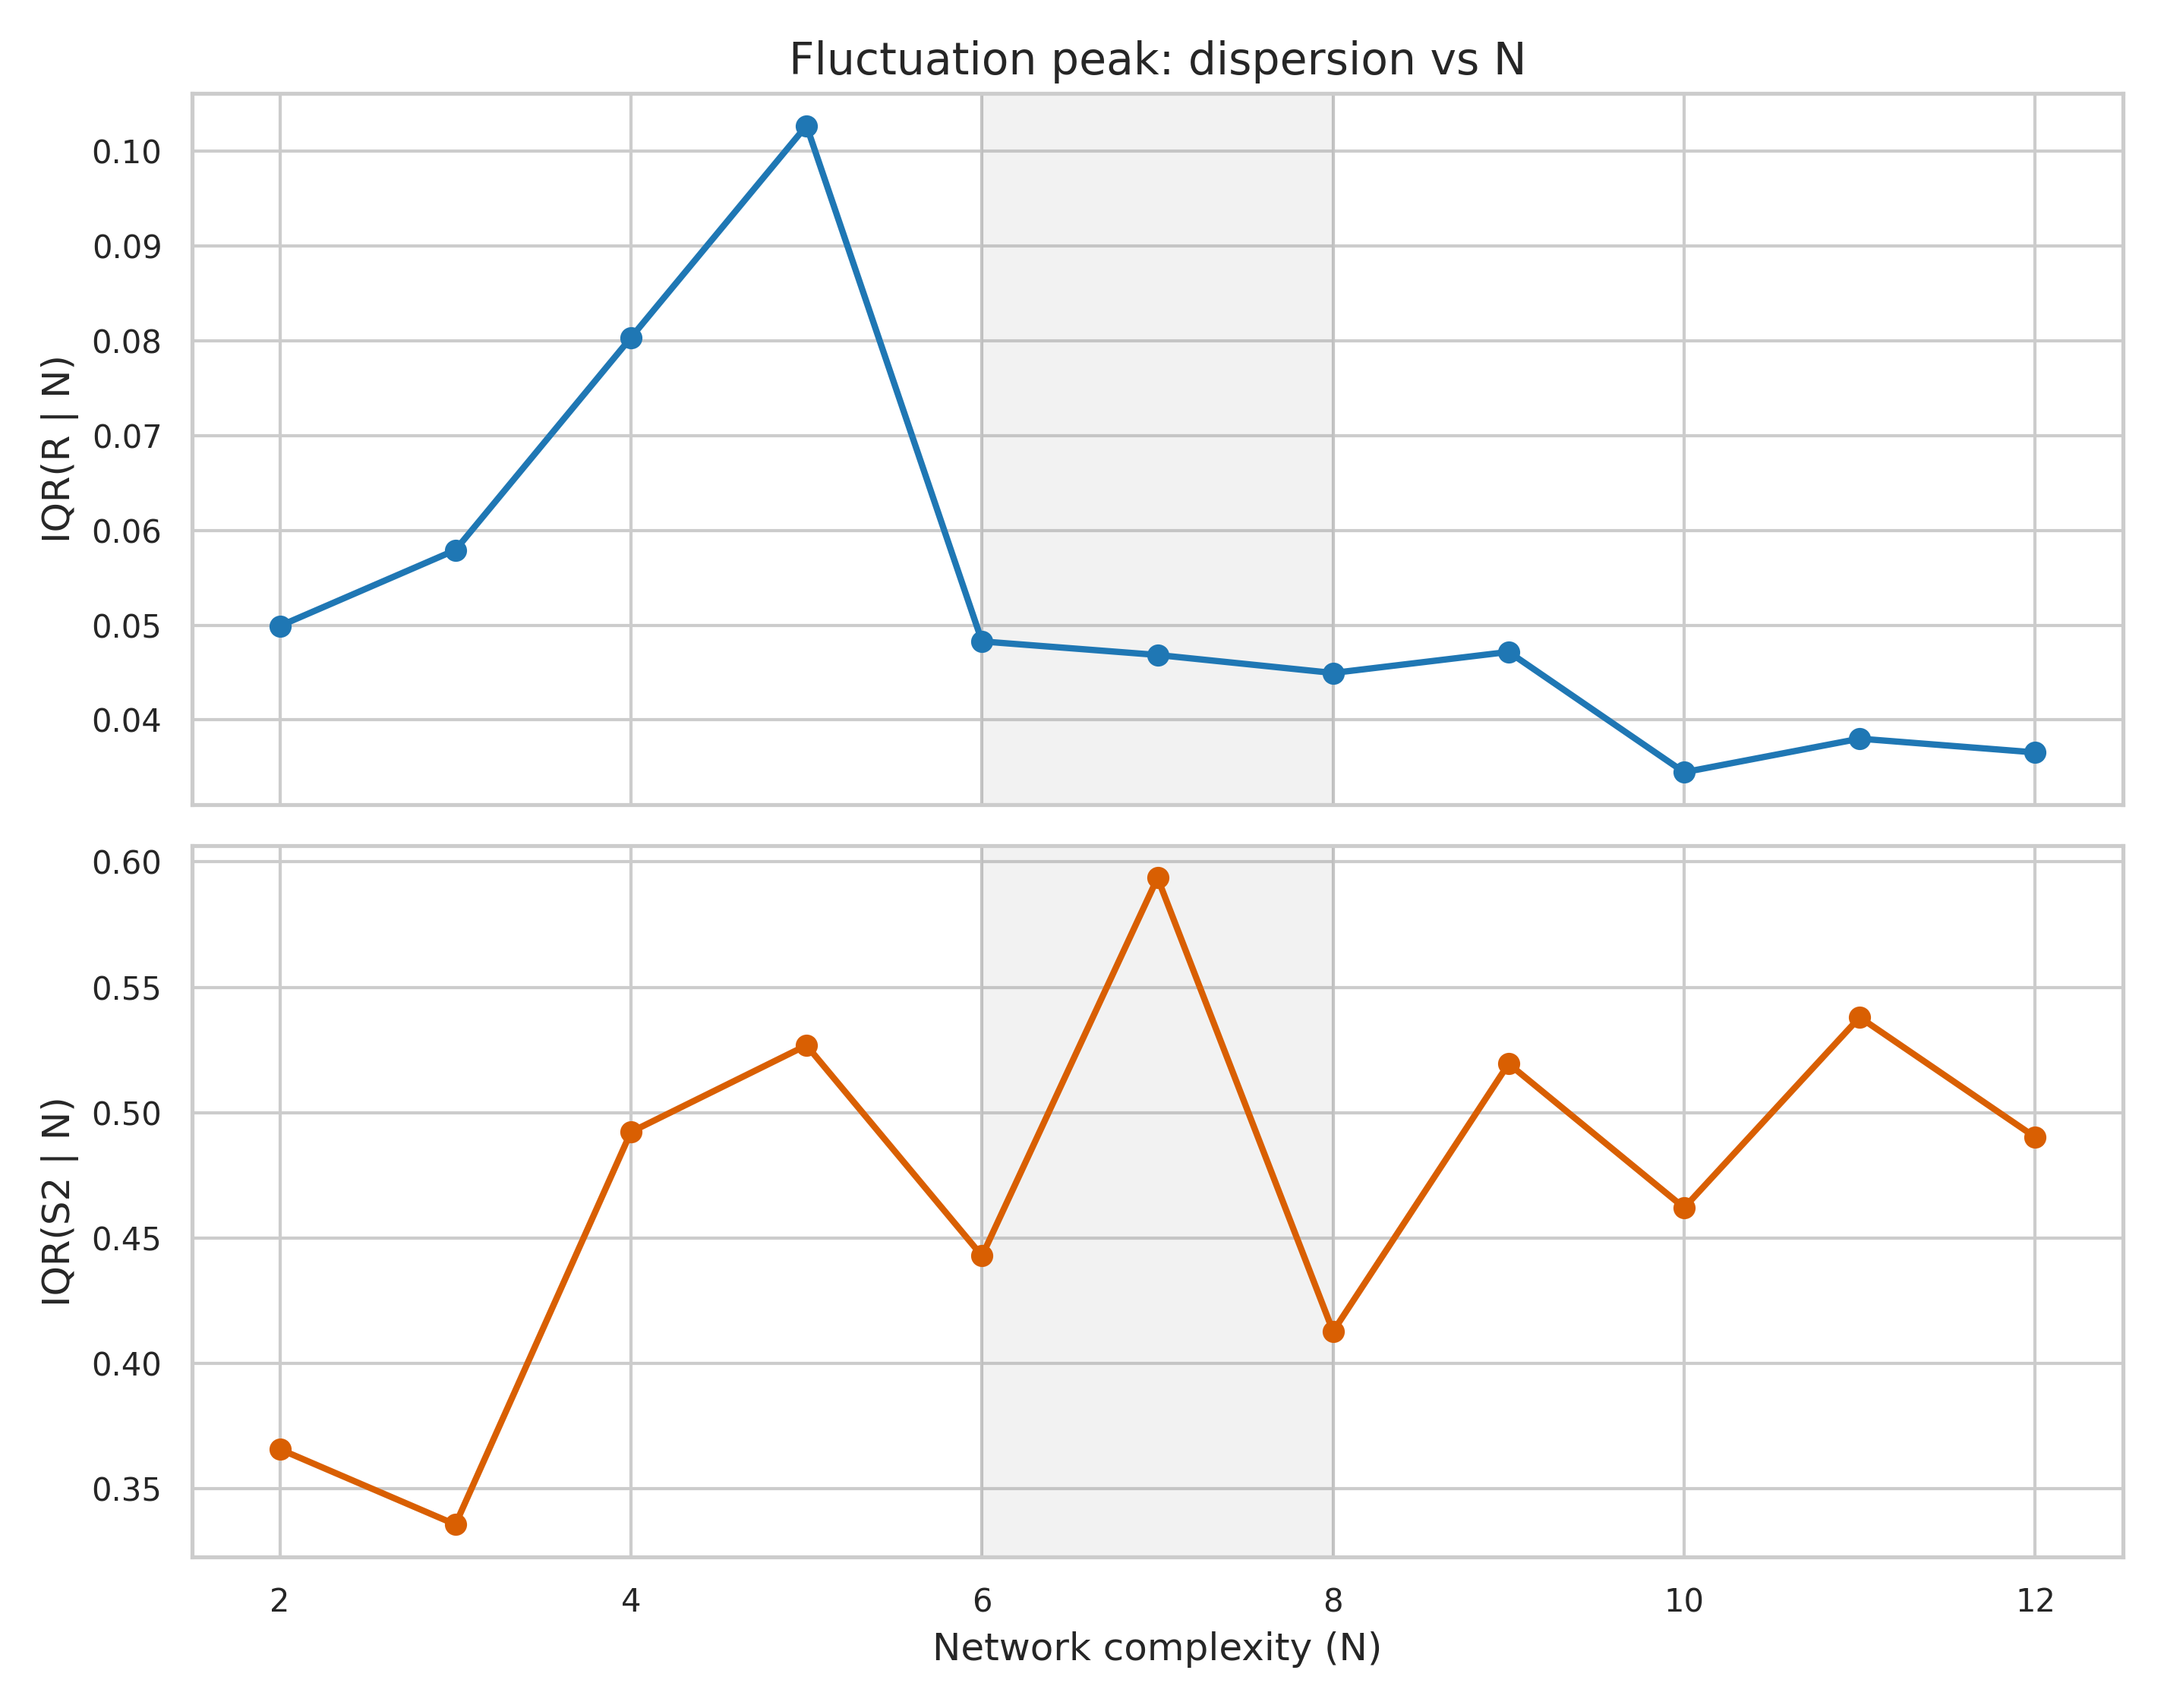
\includegraphics[width=\linewidth]{Appendix_F_Fluctuation_Peak.png}
\caption{Fluctuation peak diagnostics: dispersion vs.\ $N$.}
\label{fig:fluct}
\end{figure}

\section{Critical dynamics diagnostics}
\label{app:critical}
Figure~\ref{fig:critical} reports additional dispersion measures vs.\ $N$ used to mark the critical/transition region.

\begin{figure}[H]
\centering
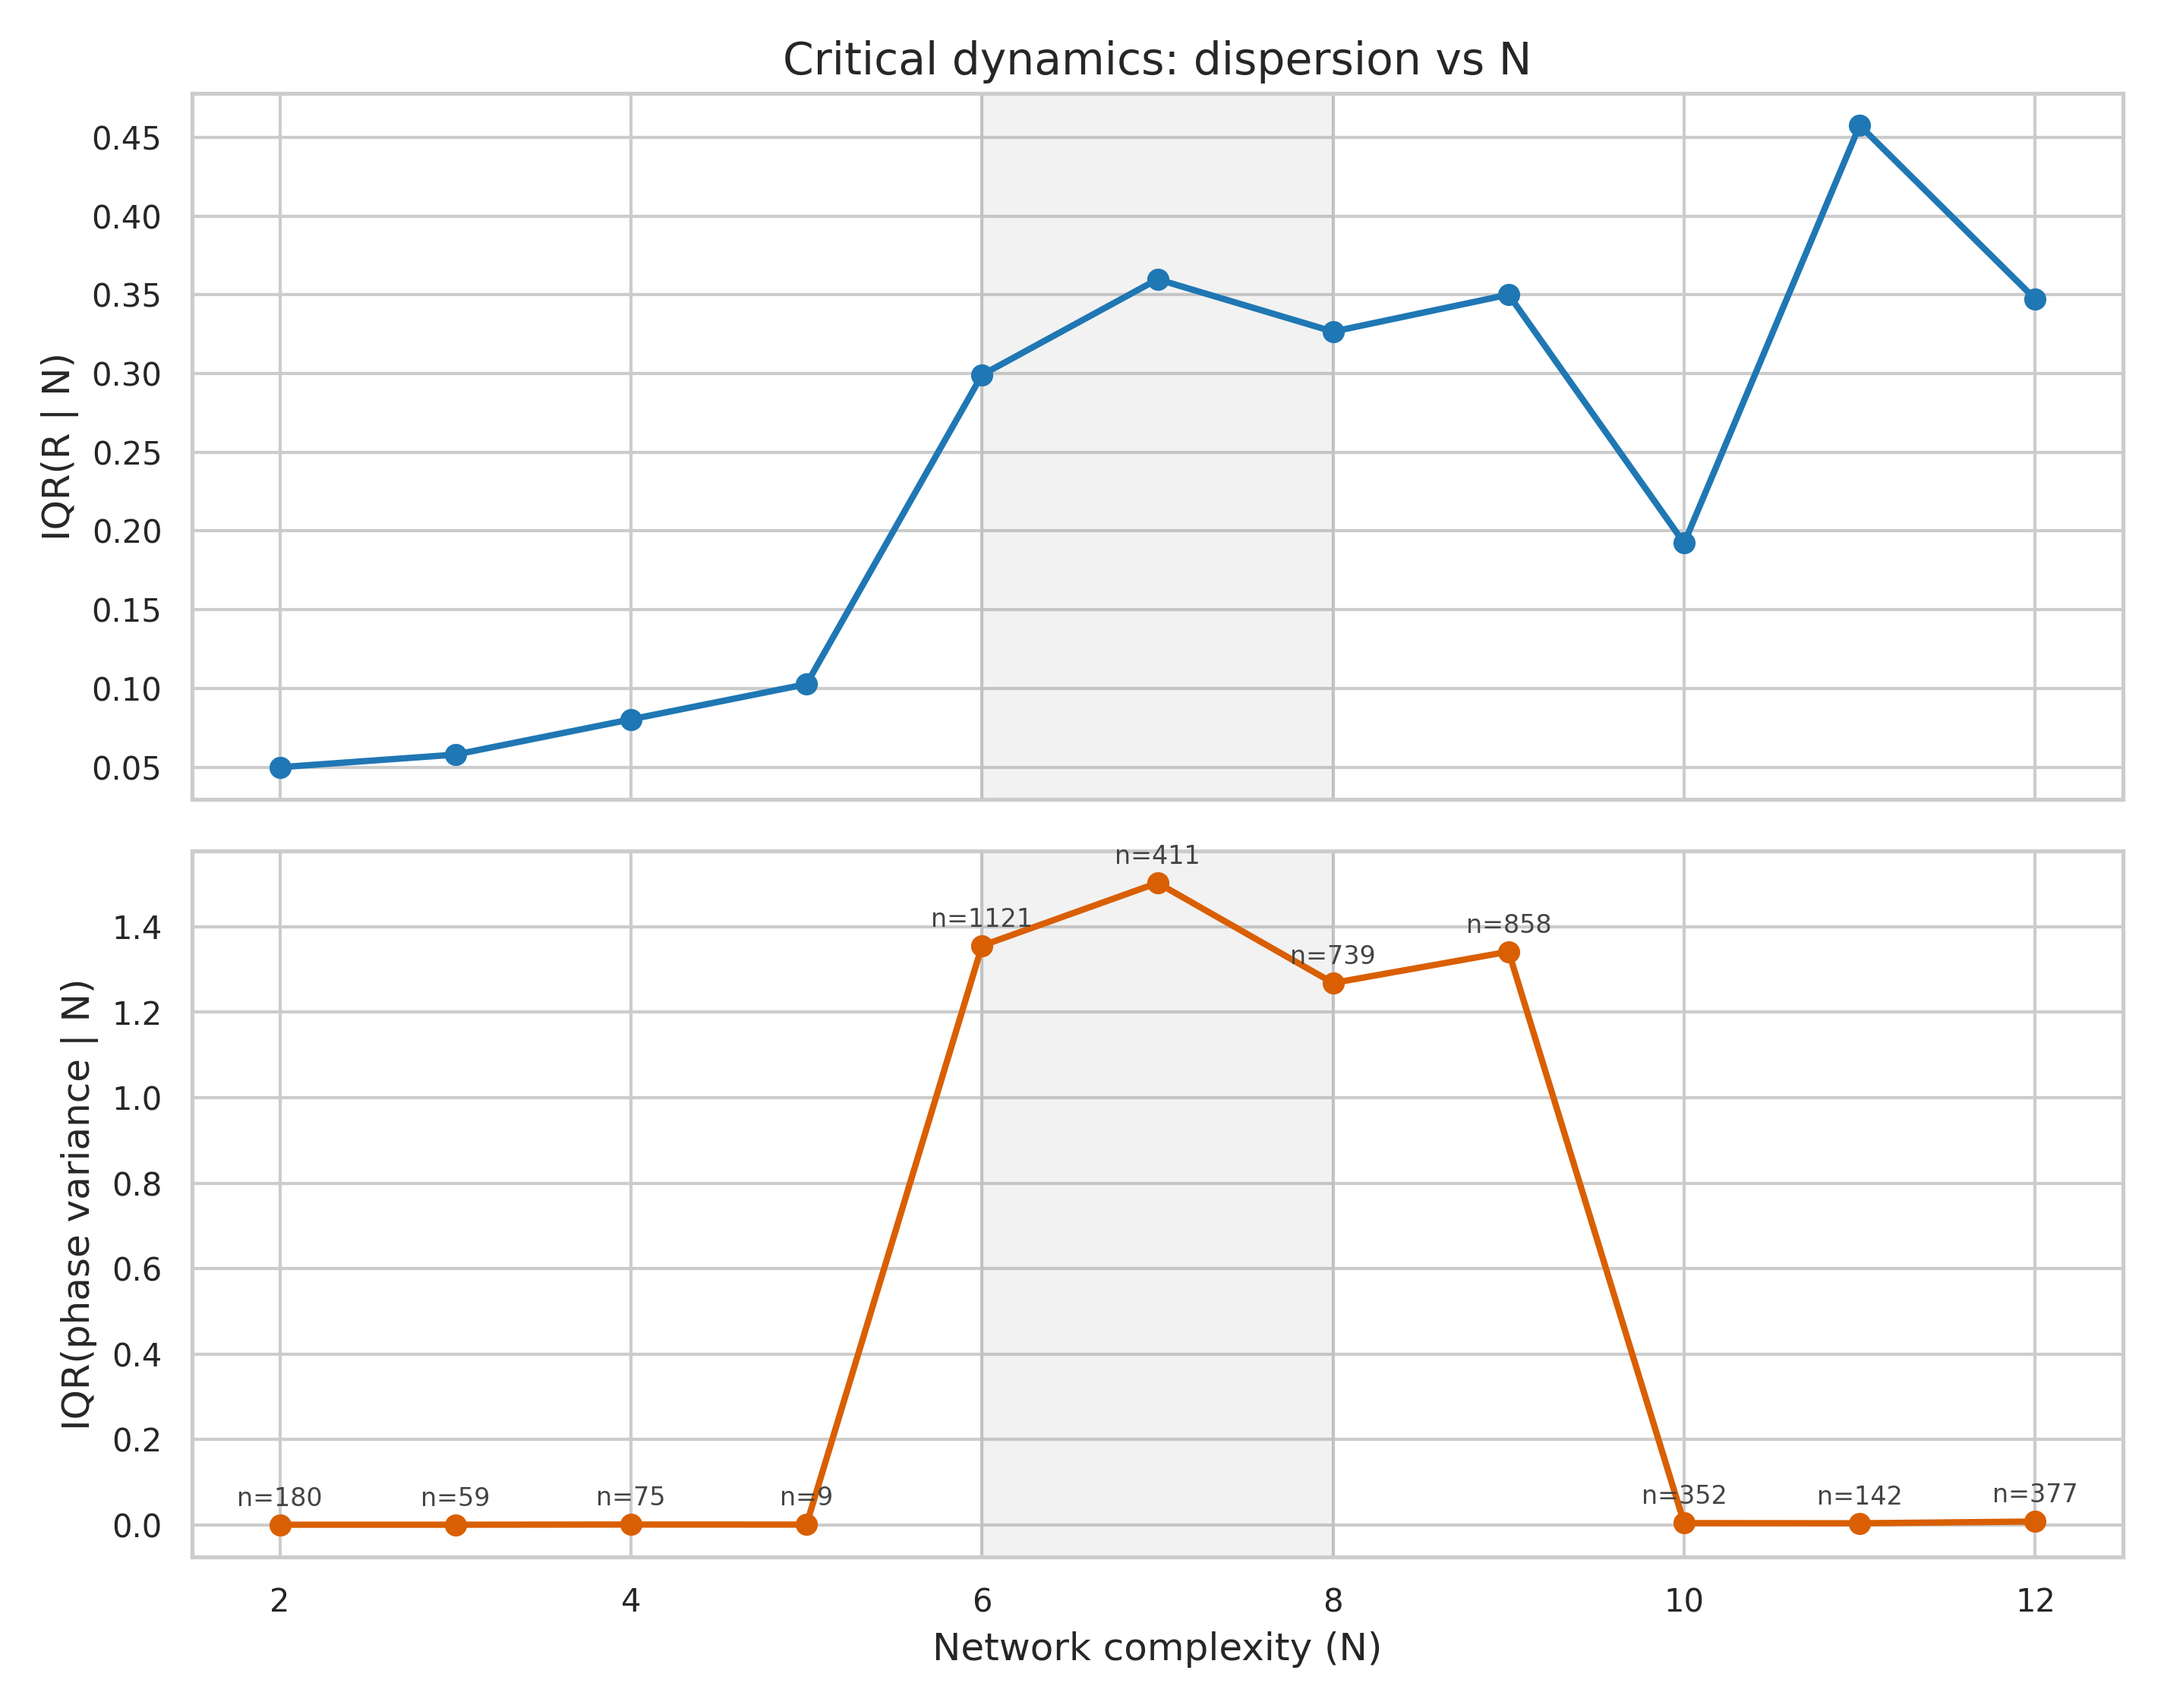
\includegraphics[width=\linewidth]{Appendix_G_Critical_Dynamics.png}
\caption{Critical dynamics diagnostics: dispersion vs.\ $N$.}
\label{fig:critical}
\end{figure}

\end{document}
